\chapter{L'importance d'une bonne gestion de la mémoire}

J'ai consacré une partie importante de mon stage à me renseigner sur l'architecture des ordinateurs et principalement comment était organisée la mémoire à l'intérieur de ces derniers. Bien comprendre comment l'ordinateur gère la mémoire est primordial pour obtenir de bonnes performances lors de l'exécution de nos programmes \cite{Drepper} (surtout lorsque plusieurs threads s'exécutent en même temps). Dans ce rapport, nous allons nous intéresser en particulier à la mémoire cache.

\section{La mémoire cache}

La mémoire cache fut développée dans les ordinateurs afin de diminuer les temps d'accès aux données stockées dans la mémoire principale. Ainsi, lorsque le processeur a besoin de données stockées dans la mémoire principale, il va réaliser une copie de celles-ci afin de les rendre plus rapidement accessibles s'ils venaient à en avoir besoin peu après. Cette amélioration est rendue possible par deux grands principes: les principes de localité spatiale et temporelle. En effet lorsqu'un programme utilise des données ou exécute des instructions, il tend à utiliser très prochainement des données ou instructions proches dans la mémoire de celles actuellement utilisées (un cas typique est la boucle \textbf{For} où les mêmes instructions seront exécutées encore et encore). \\

Le cache est généralement composé de 2 ou 3 niveaux que l'on note L1, L2 et L3. Le niveau L1, qui est le plus petit mais le plus rapidement accessible, est la plupart du temps séparé en deux parties dans un souci d'optimisation: L1d pour les copies de données et L1i pour les copies d'instructions. Le temps que met le processeur à accéder aux données présentes dans un niveau de cache croit plus ce dernier est élevé. En contrepartie, la capacité de stockage des différents niveaux de cache croit également de la même façon. \\

Afin de tenir compte du principe de localité évoqué précédemment, ce n'est pas un mot mémoire qui est chargé dans le cache mais une "ligne de cache" contenant plusieurs mots. Aujourd'hui standardisée, la taille d'une ligne de cache est de 64 octets. 

\section{Comment optimiser l'utilisation du cache}\label{Section:2.2}

En tenant compte  de ce qui a été évoqué précédemment, on peut identifier quelles sont les bonnes attitudes à adopter pour que nos programmes soient plus efficaces. Prenons l'exemple du petit programme suivant. 


\begin{DDbox}{\linewidth}
\begin{lstlisting}
#include <stdio.h>
#include <stdlib.h>

int main(){
	int tab[1000][1000];
	int i,j;

	for(i=0;i<1000;i++){
		for(j=0;j<1000;j++){
			tab[i][j] = 0;
		}
	}

	return(0);
}
\end{lstlisting}
\end{DDbox}

Dans celui-ci le tableau d'entiers à deux dimensions est parcouru séquentiellement, comme nous pouvons le voir dans la \hyperref[figure:2.1]{Figure 2.1} sur le tableau de gauche. Dans cette configuration, le processeur profite des données en cache. En effet, lorsqu'il commence à parcourir une nouvelle ligne, il extrait une ligne de cache de la mémoire principale. En considérant qu'un entier est codé sur 32 bits soit 4 octets, une ligne de cache contient donc 16 cases de notre tableau. Le processeur va donc charger des données présentes dans la mémoire cache pendant 16 itérations. \\
Supposons maintenant que nous inversons l'ordre des boucles, le schéma de parcours est à présent celui du tableau de droite de la \hyperref[figure:2.1]{Figure 2.1}. Dans cette configuration, nous ne profitons plus du cache puisque que les données chargées successivement par le processeur sont très éloignées dans la mémoire ce qui l'oblige à extraire à chaque fois une ligne de cache de la mémoire principale pour au final très peu l'utiliser. Cette version du programme est en moyenne environ 3 fois plus longue à exécuter que la précédente. 

\begin{figure}[ht]

	\begin{center}
	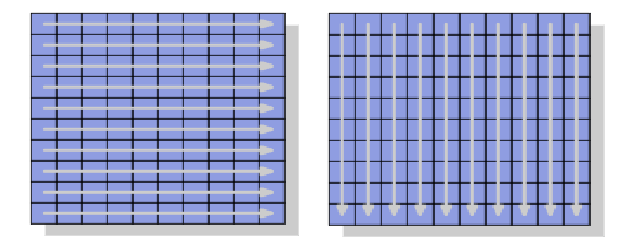
\includegraphics[scale=0.7]{tableaux.png} 
	\end{center}
	\caption{Différentes façons de parcourir un tableau}
	\label{figure:2.1}

\end{figure}

